\title{Projeto de filtro discreto passa-baixas a partir de um filtro passa-baixas Butterworth de sexta ordem}
\author{
            Aline Shayonara de Santana Ramos\\
            shayramos@hotmail.com
            \and
       	 Estev\~ao Maciel da Silva\\
       	 estevaoservo@hotmail.com
	\and
	Jo\~ao Victor Sim\~oes de Brito\\
	joao.victor.prog@gmail.com
}

\date{\today}

\documentclass[12pt]{article}

\usepackage{graphicx}
\graphicspath{ {image/} }
\usepackage[utf8]{inputenc}
\usepackage{float}
\usepackage{url}
\usepackage{amsmath}

\begin{document}
\maketitle

\noindent
Universidade Federal da Bahia\\
Profº. Antônio Carlos Lopes Fernandes Júnior\\
Processamento de sinais digitais


\section{Especifica\c c\~ao do Projeto}
\label{sec1}

Projete, a partir de um filtro passa-baixas $Butterworth$ de sexta ordem, um filtro discreto passa-baixas com fequ\^encia de corte (-3db) igual $\omega_c=2\pi/3$, usando o m\'etodo de transforma\c c\~ao bilinear. Fa\c ca a implementa\c c\~ao sob forma direta e sob forma em cascata. Represente os coeficientes em ponto flutuante (ex: $0,00423578 = 0,423578 x 10^{-2}$) e v\'a diminuindo o n\'umero de casas decimais ap\'os a v\'irgula nas formas direta e em cascata para verificar a sensibilidade \`a quantiza\c c\~ao de par\^ametros. Trace a curva do m\'odulo da resposta em frequ\^encia em dB para os casos de precis\~ao infinita e precis\~ao finita. Em seguida, para a representa\c c\~ao em forma direta, escolha duas das transforma\c c\~oes em frequ\^encia a seguir ($Z^{-1}$ = $-z^{-1}$; $Z^{-1}$ = $z^2$ ou $Z^{-1}$ = $-z^{-2}$) e trace a curva do m\'odulo em dB da resposta em frequ\^encia resultante.


\section{Filtros IIR}
\label{sec2}

Os filtros digitais s\~ao classificados pelo tipo de resposta ao impulso que apresentam como IIR(Resposta ao Impulso Infinita) ou FIR(Resposta ao Impulso Finita). Nesse trabalho ser\'a abordado o primeiro tipo de filtro, que por sua vez s\~ao recursivos, ou seja, os sinais de sa\'ida que j\'a foram calculados, far\~ao parte do c\'alculo dos sinais que ainda n\~ao foram calculados. Em geral, esses filtros possuem uma varia\c c\~ao de fase n\~ao linear.

\subsection{Butterworth}
\label{sec21}

 Este filtro \'e caracterizado por ter a magnitude da resposta plana na banda de  passagem, podendo ser utilizado no problema da aproxima\c c\~ao no projeto de filtros digitais IIR. Desse modo, \'e poss\'ivel expressar a resposta em frequ\^encia utilizando a equa\c c\~ao ~\ref{eq:1}.

\begin{equation} \label{eq:1}
|H_a(j\Omega)|^2 = \frac{1}{1+(\frac{\Omega}{\Omega_c})^{2N}}
\end{equation}

onde N \'e a ordem do filtro e  $\Omega_{c}$ a frequ\^encia de corte.

\begin{figure}[H]
\centering
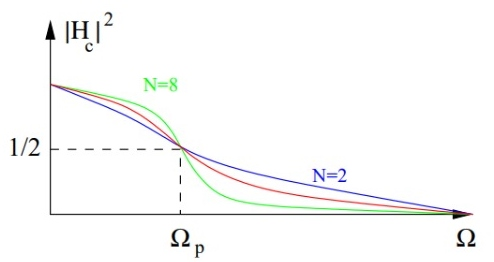
\includegraphics[width=9cm]{butter}
\caption{Resposta em frequ\^encia do filtro $Butterworth$.}
\label{butterw}
\end{figure}

\section{Transforma\c c\~ao Bilinear}
label{sec3}
\'E um dos m\'etodos usados na filtragem digital, mapeando o plano anal\'ogico $(s)$ em um plano digital $(z)$. A transforma\c c\~ao bilinear é um mapeamento matem\'atico de vari\'aveis, transformando filtros anal\'ogicos em filtros digitais equivalentes.

\begin{equation} \label{eq:2}
H(z) = H_c(s)|_{s=(\frac{2}{T_d})(\frac{1-z^{-1}}{1+z^{-1}})}
\end{equation}

onde, $H_c(s)$ é o tempo contínuo, $H(z)$ é o tempo discreto e $T_d$ o par\^ametro de amostragem. A transforma\c c\~ao bilinear imp\~oe uma rela\c c\~ao n\~ao linear entre a frequ\^encia anal\'ogica e a frequ\^encia digital, dada por $\omega = 2\tan^{-1}(\frac{\Omega}{\alpha})$, onde $\alpha= (\frac{2}{T_d})$, ou $\Omega = \alpha\tan(\frac{\omega}{2})$. Essa distor\c c\~ao \' e chamada de $warping$.


\begin{figure}[H]
\centering
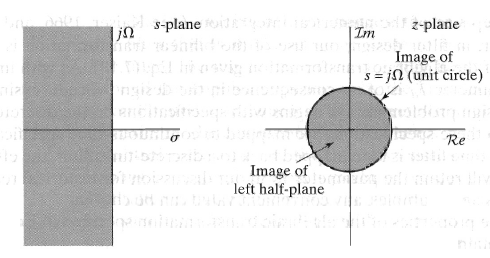
\includegraphics[width=10cm]{Omega_}
\caption{Mapeamentodo plano $s$ no plano $z$ usando transforma\c c\~ao bilinear.}
\label{map1}
\end{figure}


\begin{figure}[H]
\centering
\begin{center}
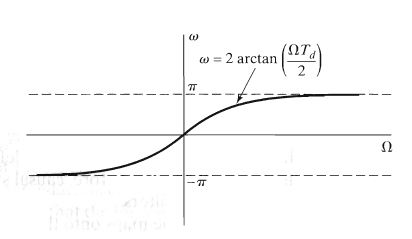
\includegraphics[width=10cm]{omega}
\end{center}
\caption{Mapeamento do eixo da frequ\^encia em tempo cont\'inuo no eixo da frequ\^encia em tempo discreto pela transforma\c c\~ao bilinear.}
\label{map2}
\end{figure}

O mapeamento entre os planos \'e, tal que, $-\infty \leq \Omega \leq \infty$ mapeado dentro de  $-\pi \leq \omega \leq \pi$.

\section{Projeto do filtro}
\label{sec4}
A ferramenta usada para o desenvolvimento do projeto foi o software MATLAB, atendendo as especifica\c c\~oes descritas na se\c c\~ao ~\ref{sec1}. Os efeitos dos processamentos no filtro foram observados com o auxilio de gr\'aficos, que ser\~ao apresentados abaixo. O primeiro passo foi gerar o filtro digital a partir do filtro passa-baixa $Butterworth$ de sexta ordem, para isso foi aplicada a transforma\c c\~ao bilinear no filtro $Butterworth$. Obteve-se a fun\c c\~ao de transfer\^encia do filtro digital na forma direta e com o numerador e denominador da mesma, foi gerado o gr\'afico da resposta em magnitude.

\begin{figure}[H]
\makebox[\textwidth]{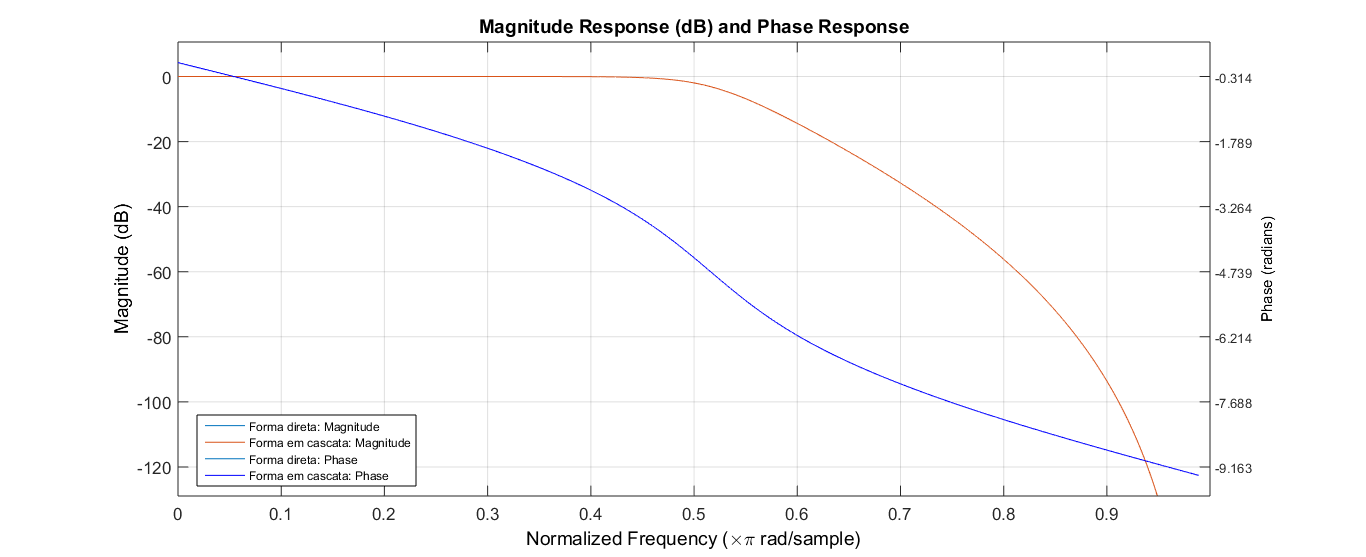
\includegraphics[width=19cm]{forma_casdir}}
\caption{Resposta em magnitude e fase na forma direta e em cascata.}
\label{casdir1}
\end{figure}


\begin{figure}[H]
\makebox[\textwidth]{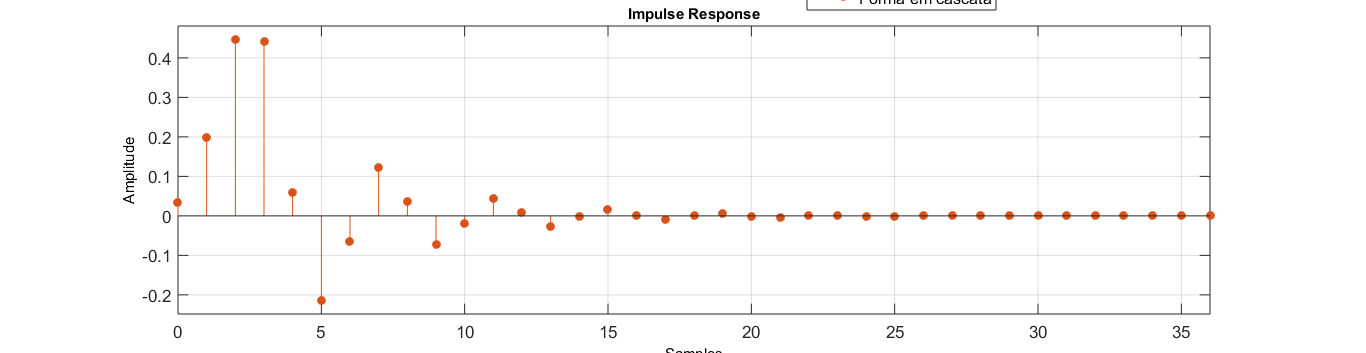
\includegraphics[width=17cm]{orig_respimp}}
\caption{Resposta ao impulso na forma direta.}
\label{respimp}
\end{figure}

A estrutura da fun\c c\~ao de transfer\^encia pode ser alterada, gerando um algoritmo diferente para o c\'alculo do mesmo sistema. A forma em cascata se d\'a pelo produt\'orio de estruturas de primeira ordem ou segunda ordem da estrutura em forma direta. Dessa forma, a partir dos polos e zeros da fun\c c\~ao de transfer\^encia na forma direta, p\^ode-se construir a estrutura na forma em cascata.

Posteriormente, foi aplicada uma manipula\c c\~ao nos coeficientes das fun\c c\~oes de transfer\^encia de ambas estruturas discutidas acima, diminuindo o n\'umero de casa decimais dos coeficientes gradativamente, com o intuito de observar a sensibilidade a quantiza\c c\~ao de par\^ametros da forma direta e cascata, separadamente. 
Na implementa\c c\~ao do filtro, o MATLAB retorna os coeficientes com precis\~ao de 15 casas decimais, chamada de precis\~ao infinita. Nesse trabalho, foram feitas aproxima\c c\~oes usando entre tr\^es e uma casa decimal, chamada de precis\~ao finita. Como seguem  nos gr\'aficos abaixo:

\begin{figure}[H]
\makebox[\textwidth]{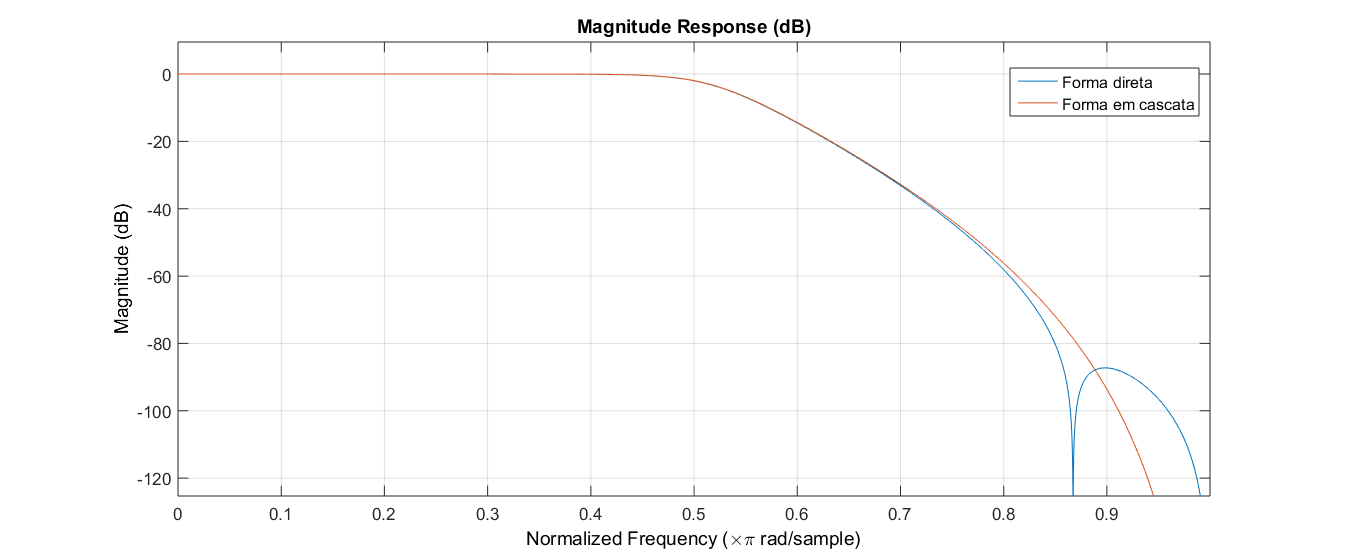
\includegraphics[width=19cm]{forma_casdir3}}
\caption{Resposta em magnitude e fase na forma direta e em cascata com precis\~ao de 3 casas decimais.}
\label{casdir2}
\end{figure}

\begin{figure}[H]
\makebox[\textwidth]{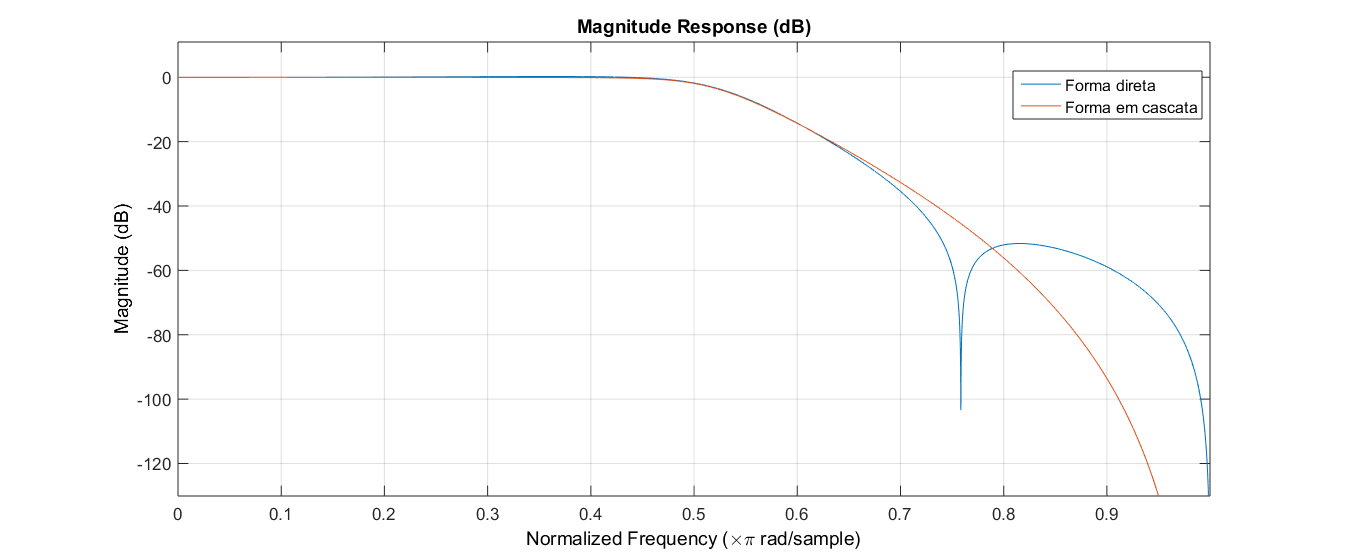
\includegraphics[width=19cm]{forma_casdir2}}
\caption{Resposta em magnitude e fase na forma direta e em cascata com precis\~ao de 2 casas decimais.}
\label{casdir3}
\end{figure}

\begin{figure}[H]
\makebox[\textwidth]{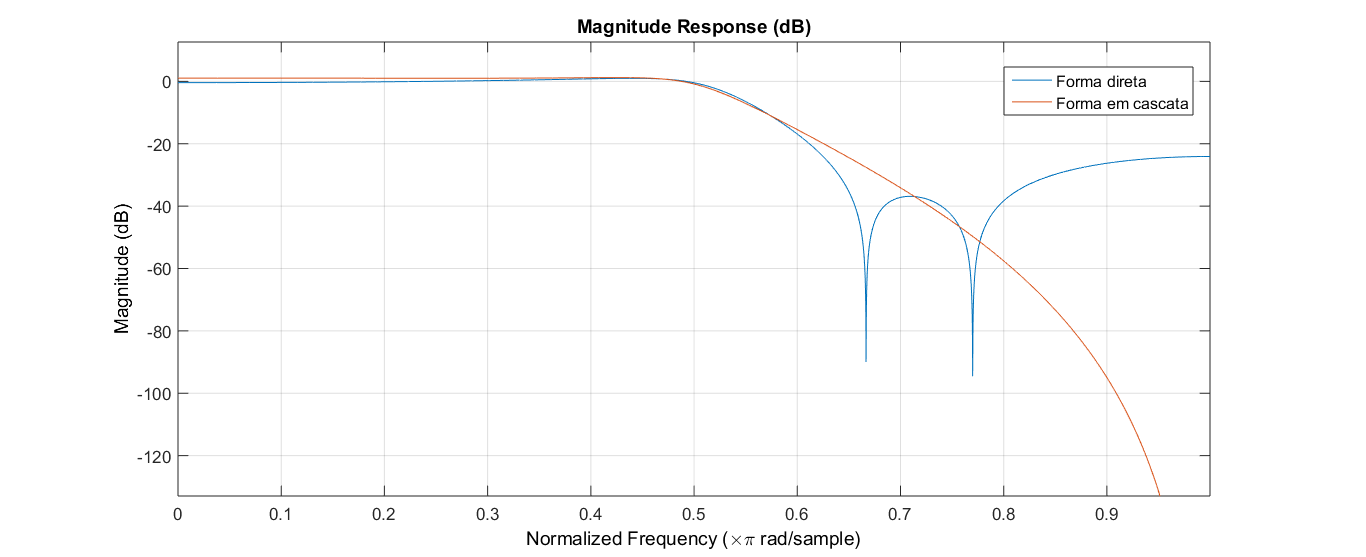
\includegraphics[width=19cm]{forma_casdir1}}
\caption{Resposta em magnitude e fase na forma direta e em cascata com precis\~ao de 1 casa decimal.}
\label{casdir4}
\end{figure}

Da mesma forma foi feito para o m\'odulo da resposta em frequ\^encia. Fazendo um comparativo entre o gráfico da forma direta e em cascata no caso de precis\~ao infinita, tanto na figura \ref{casdir1}, como na figura \ref{precisao_infinita}, \'e poss\'ivel notar que os gr\'aficos n\~o diferem uns dos outros, isso acontece porque, nesse caso a precis\~ao dos coeficientes de ambas estruturas s\~ao altas (15 casas decimais).

\begin{figure}[H]
\makebox[\textwidth]{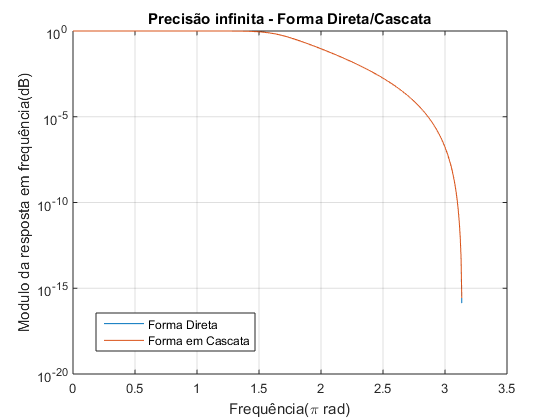
\includegraphics[width=10cm]{precisao_infinita}}
\caption{Módulo da resposta em frequ\^encia na forma direta e cascata com precis\~ao infinita.}
\label{precisao_infinita}
\end{figure}

Nos casos de precis\~ao finita, pode-se perceber, tantos nos gr\'aficos de resposta em magnitude quanto nos de m\'odulo da resposta em frequ\^encia, que a forma direta \' e mais sens\' ivel a quantiza\c c\~ao de par\^ametros do que a forma em cascata, ou seja, os erros de quantiza\c c\~ao dos coeficientes dos filtros s\~ao menos severos para a implementa\c c\~ao em cascata. Por isso estruturas na forma direta, em geral, n\~ao s\~ao  recomendadas em aplica\c c\~oes pr\'aticas, em contrapartida percebe-se que o filtro nessa estutura tem uma menor banda de transi\c c\~ao.

\begin{figure}[H]
\makebox[\textwidth]{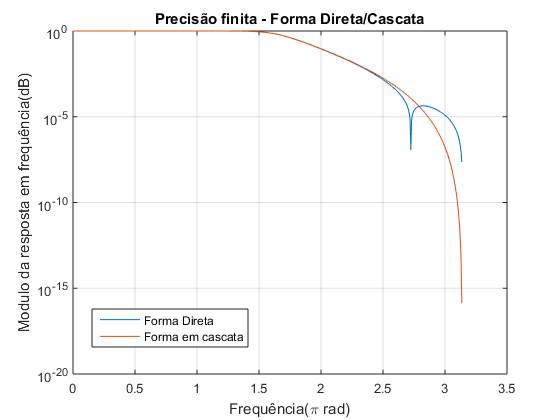
\includegraphics[width=10cm]{precisao_finita3}}
\caption{Módulo da resposta em frequ\^encia na forma direta e cascata com precis\~ao finita de 3 casas decimais.}
\label{precisao_finita3}
\end{figure}

\begin{figure}[H]
\makebox[\textwidth]{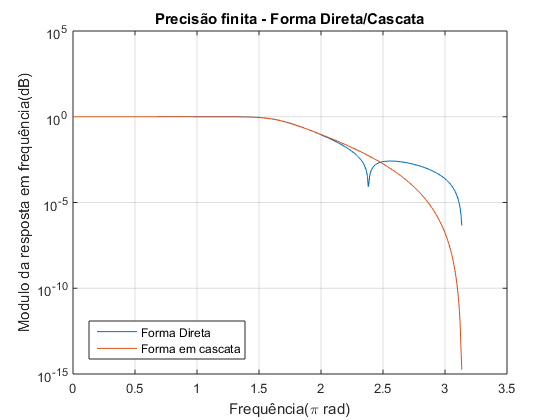
\includegraphics[width=10cm]{precisao_finita2}}
\caption{Módulo da resposta em frequ\^encia na forma direta e cascata com precis\~ao finita de 2 casas decimais.}
\label{precisao_finita2}
\end{figure}

\begin{figure}[H]
\makebox[\textwidth]{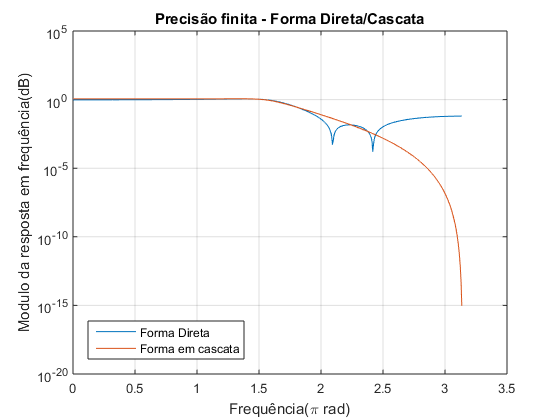
\includegraphics[width=10cm]{precisao_finita1}}
\caption{Módulo da resposta em frequ\^encia na forma direta e cascata com precis\~ao finita de 1 casa decimal.}
\label{precisao_finita1}
\end{figure}

Dessa forma pode-se confirmar que quando o n\'umero de polos \'e grande, uma pequena mudan\c ca em um coeficiente do filtro devido ao par\^ametro de quantiza\c c\~ao resulta em uma grande mudan\c ca na loca\c c\~ao dos polos e zeros do sistema.

\subsection{Transforma\c c\~ao em frequ\^encia}

A transforma\c c\~ao em frequ\^encia tem o intuito de modificar as caracter\'isticas do filtro atrav\'es de uma transforma\c c\~ao em $z$, de foma que:

\[H(z) = H_{lp}(Z)|_{Z^{-1}=G(z^{-1})}\]
 
onde $H_{lp}(Z)$ \'e um sistema passa-baixas, no qual deseja-se transformar para um sistema $H(z)$ de outra natureza. O mapeamento deve ser tal que, a estabilidade do filtro seja mantida, isso equivale dizer que a transforma\c c\~ao mapeia o interior do c\'irculo unit\'ario para o interior do c\'irculo unit\'ario, e o exterior do c\'irculo unit\'ario para o exterior do c\'irculo unit\'ario.

\subsubsection{$Z^{-1}$ por $-z^{-1}$}
\label{subsec411}
Com essa transforma\c c\~ao na fun\c c\~ao de transfer\^encia do filtro passa-baixa, foi poss\'ivel observar que o mesmo se transformou em um filtro passa-alta, com as mesmas especifica\c c\~oes do filtro antigo.

\begin{figure}[H]
\makebox[\textwidth]{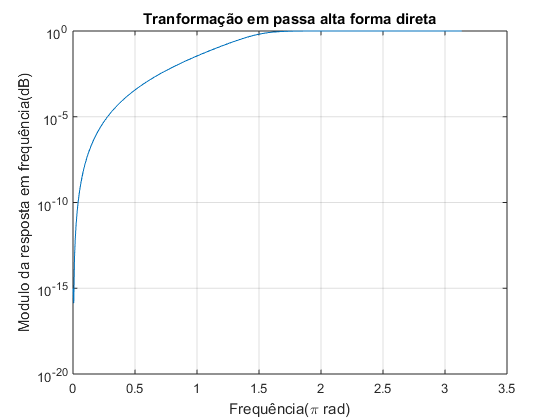
\includegraphics[width=10cm]{passa_alta}}
\caption{Módulo da resposta em frequ\^encia na forma direta, transforma\c c\~ao em passa alta}
\label{passa_alta}
\end{figure}

No que diz respeito a resposta ao impulso, a transforma\c c\~ao em frequ\^encia acarretou na altera\c c\~ao dos sinais de alguns coefecientes para o sinal negativo, percebe-se isso comparando a figura \ref{respimp} e a figura \ref{passa_alta2}.

\begin{figure}[H]
\makebox[\textwidth]{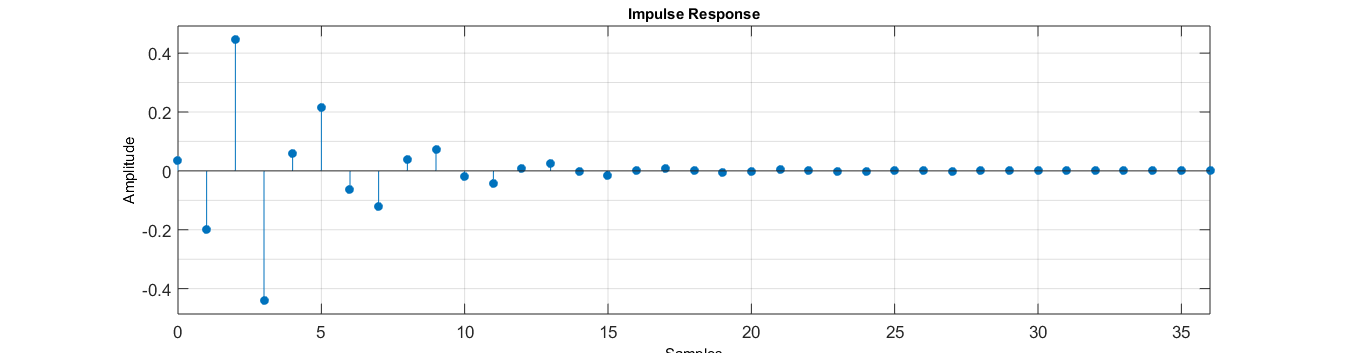
\includegraphics[width=17cm]{passa_alta_frequency}}
\caption{Resposta ao impulso na forma direta, passa alta}
\label{passa_alta2}
\end{figure}

\subsubsection{$Z^{-1}$ por $-z^{-2}$}

Diferente da se\c c\~ao ~\ref{subsec411} o filtro tornou-se passa-faixa, preservando as especifica\c c\~oes iniciais do filtro.

\begin{figure}[H]
\makebox[\textwidth]{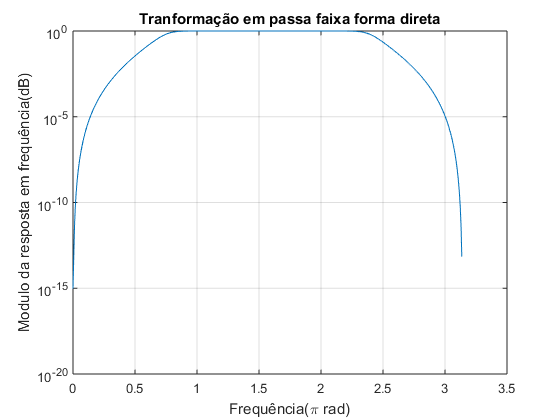
\includegraphics[width=10cm]{passa_faixa}}
\caption{Módulo da resposta em frequ\^encia na forma direta, transforma\c c\~ao em passa faixa}
\label{passa_faixa}
\end{figure}

Observando a figura ~\ref{respimp} e a figura ~\ref{passa_faixa2}, nota-se que al\'em da negativa\c c\~ao, a transforma\c c\~ao dobra a ordem dos coeficientes do filtro, ocorrendo uma expans\~ao dos registradores de deslocamento no eixo das frequ\^encias 

\begin{figure}[H]
\makebox[\textwidth]{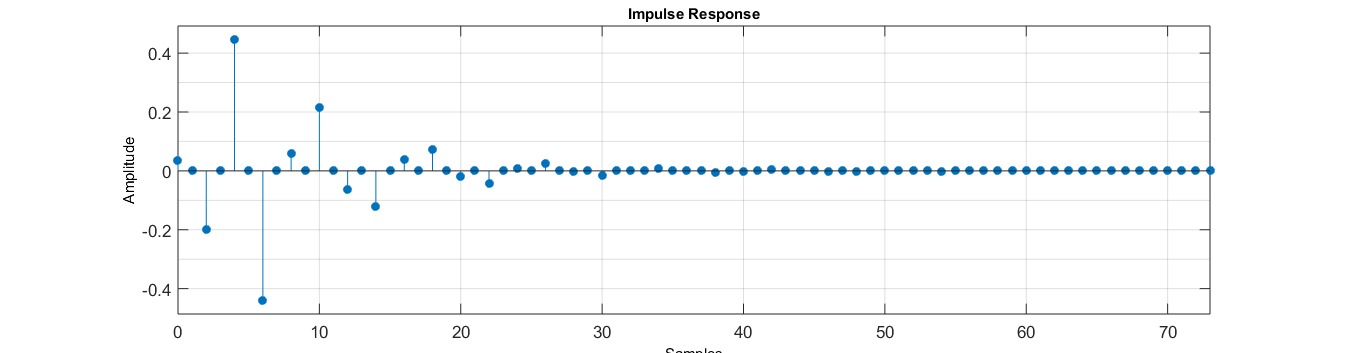
\includegraphics[width=17cm]{passa_faixa_frequency}}
\caption{Resposta ao impulso na forma direta, passa faixa}
\label{passa_faixa2}
\end{figure}

\bibliographystyle{abbrv}
\bibliography{simple}

\end{document}